\chapter{Experiment and Results}

he proposed face de-identification approach has been implemented. Recently, I spend most time in setting up experiments and the corresponding analysis. This report would display the de-identified face images in both shape and appearance level. To inspect the ability of protecting privacy, face recognition algorithm is applied to the original face images and de-identified results. On the other hand, expression recognition algorithm is used to check whether the approaches are able to preserve the useful information.  


\section{De-identified results}
In our experiment, CMU PIE face database is firstly used to test the proposed approaches. Images from 20 subjects are chosen to build the tensor model. Each one of them has 3 poses: frontal, left profile, right profile, and 2 expressions: normal and smile. Other images are for testing. The program is executed in Matlab. The Sandia tensor toolbox is used to analyze the tensor. To show the flexibility of our proposed framework, another face database, IMM, is also tested. The types of pose and expression involved in IMM are the same as CMU PIE, but there are no smile images for right profile and left profile poses. Therefore, expression dimension is not included in IMM experiment. 

A face image is processed in two levels: shape and appearance. Similar with AAM, the feature points in one face compose its shape. Different faces in different poses yield a unique shape. The de-identified algorithms could transform a shape into a different one that represents a similar pose. Appearances are the pixels in an image. The de-identified appearance is expected to be different and normal. In plain words, the result face is normal looking. No distortion or other unnatural appearance would show. The most important is people could not recognize the person identity in results based on original images.


	\subsection{Proposed approach}

	All the group images appear in this report is arranged as: the right is the original image and the left is de-identified result. Fig.\ref{fig:shape_recon} is a sample of shape de-identification. The shape data has been decomposed into multiple dimensions and we only modify the identity one, so the result is not the same with original shape but is in similar pose.

	\begin{figure}[!htb]
		  \centering
		  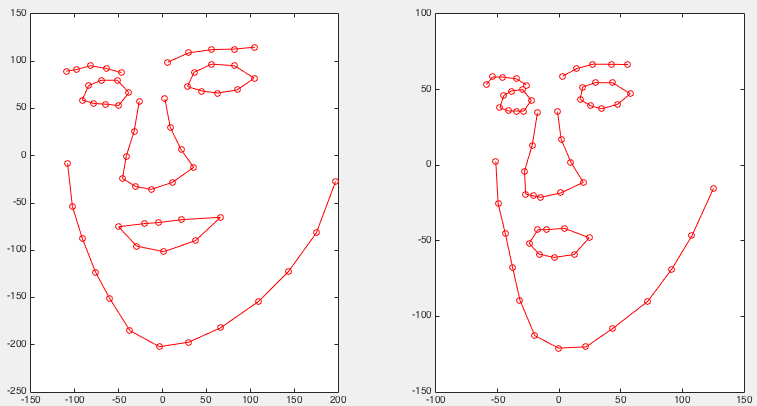
\includegraphics[width=0.6\textwidth]{figure/shape_recon}
		  \caption{Shape de-identification by proposed approach}
		  \label{fig:shape_recon}
	\end{figure}

	For the face shapes are not in the same size, all appearances are warped to a mean shape so that it is possible to compare different images. Therefore, the de-identified appearance should warp back to de-identified shape. That is the final result of our approach. Fig. \ref{fig:tensor_result_1} is one example of final result.

		\begin{figure}[!htb]
		  \centering
		  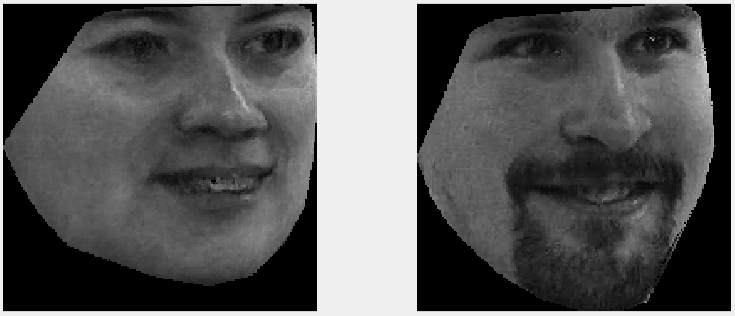
\includegraphics[width=0.6\textwidth]{figure/right_smile}
		  \caption{De-identified appearance warp back to de-identified shape}
		  \label{fig:tensor_result_1}
		\end{figure}

	The criteria of judgeing the result are:
	\begin{enumerate}
		\item the de-identified face is not the same one with the original face,
		\item the de-identified face is normal, containing no unnatural appearance like distortion.
	\end{enumerate}


	\subsection{k-same-M}
	K-same-M is one of the best face de-identification algorithms. It describes a face image by parameters of a model like AAM and then take the average of $k$ image parameters as a new one. At last, a new face image is reconstructed by the new parameters and the model. Since all parameters are in the same dimension, the result might lose more useful information than identity. Fig. \ref{fig:shape_k_s} is an example of shape de-identification. The original left profile pose is tranformed into frontal face. 

	\begin{figure}[!htb]
	  \centering
	  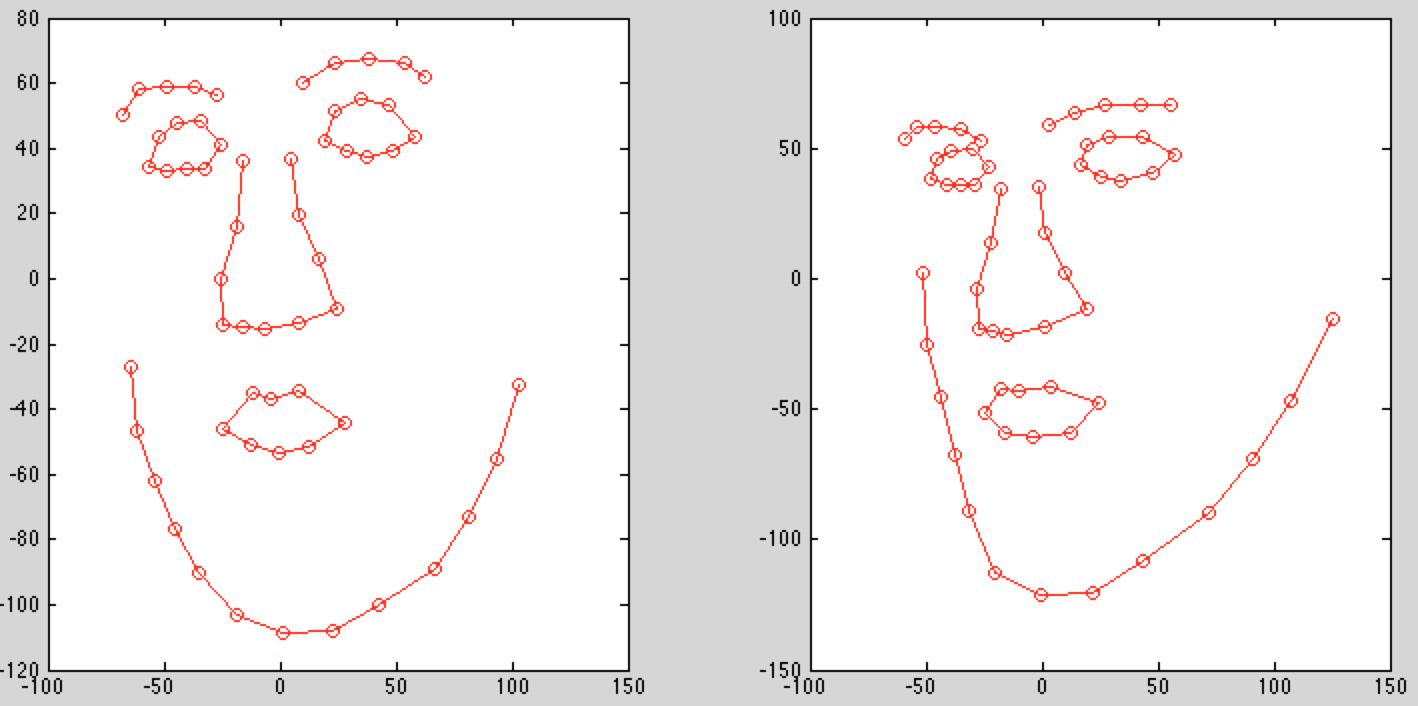
\includegraphics[width=0.6\textwidth]{figure/model_shape_1}
	  \caption{shape de-identification by k-same-M}
	  \label{fig:shape_k_s}
	\end{figure}

	De-identified appearance that warps back to de-identified shape forms the final result. If the face shape has been tranformed into a wrong one, the final result must be distorted and unnatural. Fig. \ref{fig:MkS} is an example of model-based de-identification results. The result has an obvious distortion in the face. 

	\begin{figure}[!htb]
	  \centering
	  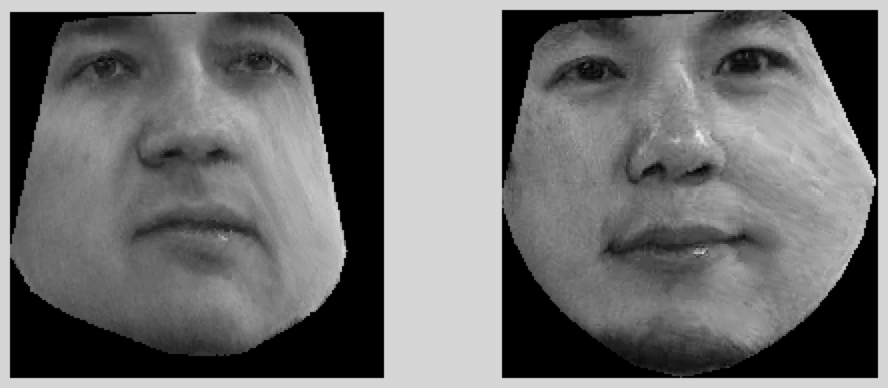
\includegraphics[width=0.6\textwidth]{figure/model_result}
	  \caption{de-identification by k-same-M}
	  \label{fig:MkS}
	\end{figure}

	K-same-M can definitely produce good results like Fig.\ref{fig:model_result}. However, the data utility of de-identified results can not be guaranteed. 

		\begin{figure}[!htb]
		  \centering
		  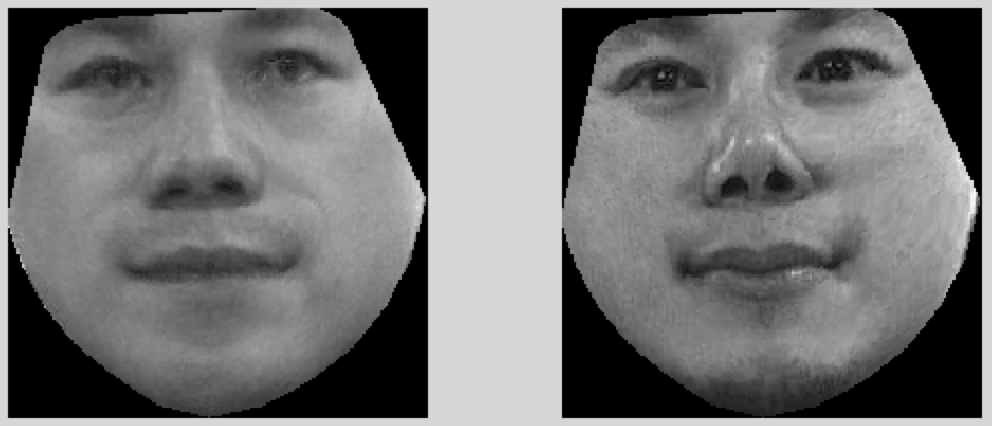
\includegraphics[width=0.6\textwidth]{figure/good_MkS}
		  \caption{model k same}
		  \label{fig:model_result}
		\end{figure}

\section{Recognition}

We have compared the proposed approach and existing ones in human vision level. The key point in face de-identification is to keep the ballance between privary protection and data utility preservation. We have addressed the expression is the most importatn information.This section would examine privacy and expression preservation in quantity.
	
	
	\begin{figure}[!htb]
	  \centering
	  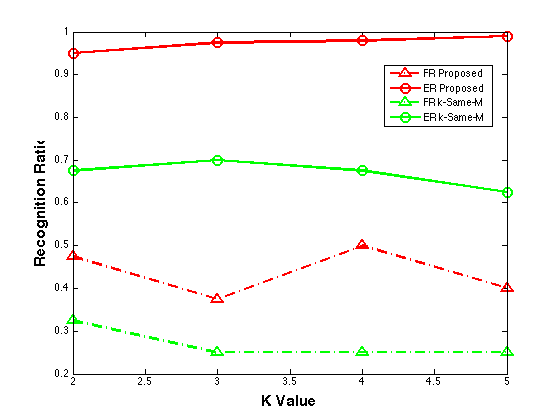
\includegraphics[width=0.8\textwidth]{figure/plotPic}
	  \caption{Recognition ratio.}
	  \label{fig:plotPic}
	\end{figure}

	Only frontal face images are used because the recognition algorithms performs best in these images. The PCA+KNN is chosen as the inspection method for face recognition (FR) and expression recognition (ER). This is the most stable recognition framework. Furthermore, it is easy to implement and performs well in small dataset. I think the inpsection method is not the key point of this experiment. It is the comparisons that really matter. 

	From the Fig. \ref{fig:plotPic}, we can see FR ratio of proposed approach is higher than k-same-M, but it is still acceptable. The ER ratio of proposed approach is increased to a high level. It is a trade-off between privacy and data utility. Our target is to preserve the data utility as large as possible when the privacy is protected well. 



The above is the objective testing. Further work about subjective testing is being prepared. I would design some questionnares for a survey about FR of de-identified results. 
